\begin{figure}[H]
    \begin{subfigure}[t]{\textwidth}
        \caption{}
        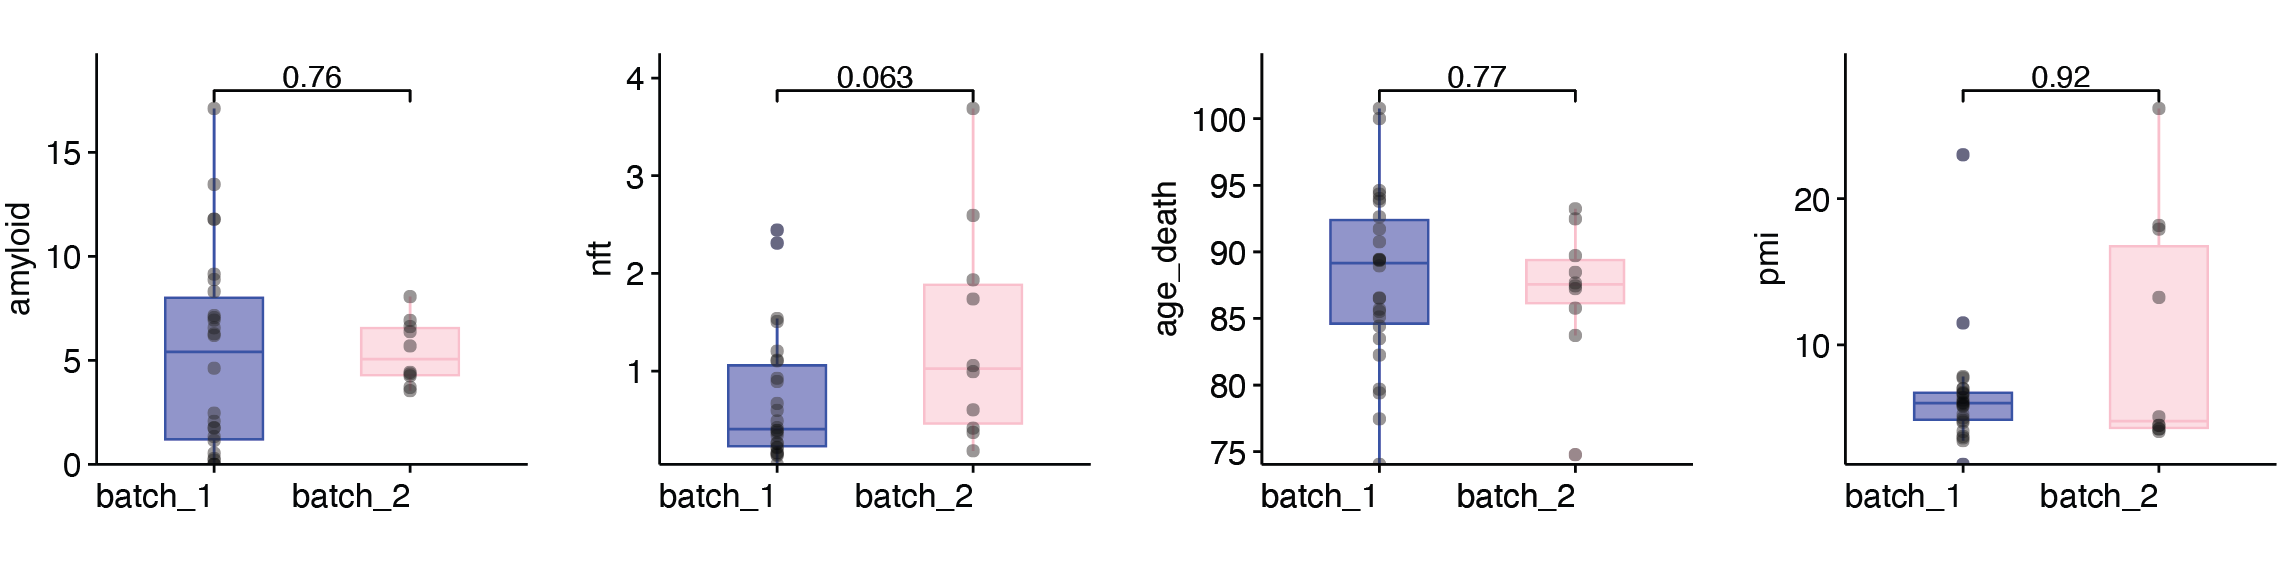
\includegraphics[width=\textwidth]{./extended_plots/seq_batch_cont.png}        
    \end{subfigure}
    \begin{subfigure}[t]{\textwidth}
        \caption{}
        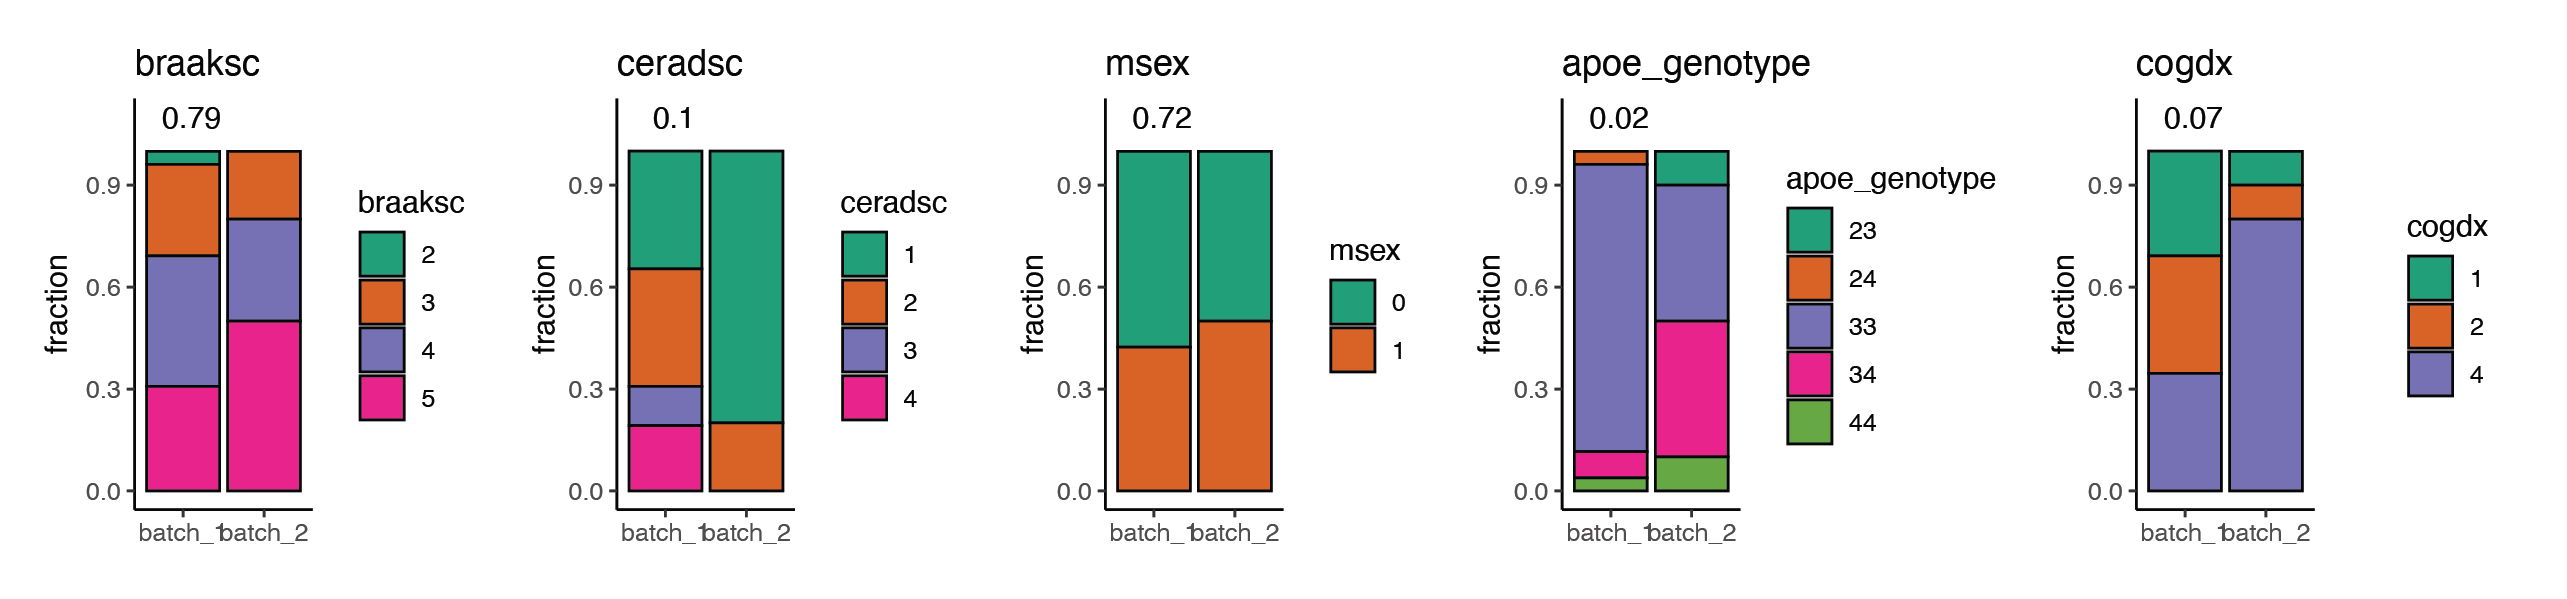
\includegraphics[width=\textwidth]{./extended_plots/seq_batch_cat.png}        
    \end{subfigure}  
    \begin{subfigure}[t]{\textwidth}
        \caption{}
        \includegraphics[width=\textwidth]{./extended_plots/additional_projections.png}        
    \end{subfigure}   
    \begin{subfigure}[t]{\textwidth}
        \caption{}
        \includegraphics[width=\textwidth]{./extended_plots/score_correlations_by_batch.png}        
    \end{subfigure}   
    \caption{
        \textbf{Overview of snRNA-sequencing Batch Correction and Data Quality.}\\
    }
    \label{fig:snRNA_batch_quality}
\end{figure}
\begin{itemize}
    \item[\textbf{(A)}] Distribution of continuous metadata variables by sequencing batch. P-values in panels were computed by two-sided Wilcoxon rank sum test.
    \item[\textbf{(B)}] Distribution of discrete metadata variables by sequencing batch. P-values were computed by two-sided Fisher's exact test.
    \item[\textbf{(C)}] 2D UMAP projection of snRNA-seq cells after quality control, colored by selected metadata variables.
    \item[\textbf{(D)}] Correlation of gene perturbation scores ($S = -\log_{10}(p)\times\text{sign}(\log_2(\text{fold-change}))$) computed using all samples versus excluding batch 2 (v2 chemistry), demonstrating that results are robust and not driven by batch-specific effects.
\end{itemize}